\subsection{Clave-Valor}

\begin{frame}
    \frametitle{Clave-Valor - Repaso}

    Este modelo almacena pares del tipo (\textit{Key}, \textit{Value}).
    
    \begin{center}
    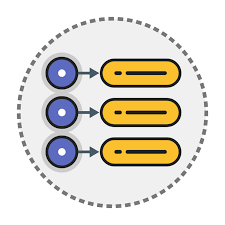
\includegraphics[width=0.2\textwidth]{images/KeyValue.png}
    \end{center}

     
    
     \begin{itemize}
        \item \textbf{Key}: Un identificador único para acceder al valor asociado.

         
        
         \item \textbf{Value}: Puede ser cualquier tipo de dato, desde texto, números y documentos, hasta listas o incluso otros pares clave-valor.
     \end{itemize}

\end{frame}

\begin{frame}
    \frametitle{Clave-Valor - Ejemplos}
    
    Algunas de las implementaciones más conocidas son:

     
    
     \begin{itemize}
        \item \textbf{Amazon DynamoDB}
                        
        \item \textbf{Voldemort}

        \item \textbf{Riak}
        
        \item \textbf{Redis}
     
     \end{itemize}

     

     Nos vamos a centrar en esta última.
\end{frame}

\subsubsection{Redis}

\begin{frame}   
    \frametitle{Clave-Valor - Redis}

    \textbf{Redis} significa ``\textbf{RE}mote \textbf{DI}ctionary \textbf{S}erver''

    \begin{center}
        
\includegraphics[width=0.3\textwidth]{images/redis_logo.png}
    \end{center}
    
     

    \begin{itemize}
        \item Base de datos de código abierto.  
        \item Rápida y versátil.  
        \item Diseñada como un almacén de estructuras de datos en memoria.
    \end{itemize}

\end{frame}

\begin{frame}
    \frametitle{Características de Redis}

    \begin{itemize}
        \item Estructuras de datos: strings, hashes, listas, conjuntos, etc.  
        \item Operaciones atómicas: Agregar, incrementar, intersección, unión, etc.  
        \item Replicación de datos incorporada.  
        \item Trabaja con un conjunto de datos en memoria.
    \end{itemize}
\end{frame}

\begin{frame}{Operaciones de Redis}
    
    Redis ofrece más de \textbf{400} operaciones e implementa la interfaz teórica para cada uno de los tipos de datos mencionados.
    
      

    Algunos ejemplos son:

      

    \begin{itemize}
        \item \textit{Strings:} $SET$, $GET$ y $DEL$
        
        \item \textit{Hashes:} $HSET$, $HGET$ y $HDEL$

        \item \textit{Listas:} $LPUSH$, $LPOP$, $RPUSH$, $RPOP$, $LRANGE$

        \item etc.
    \end{itemize}

\end{frame}

\begin{frame}{Ejemplo de Uso}
    \textbf{SET}: Agrega un par $(key, value)$.
    \begin{itemize}
        \item Complejidad temporal: $\mathcal{O}(1)$.
    \end{itemize}
    \vspace{0.6}
    \texttt{redis> SET subject1 "Base de Datos Avanzadas"} \newline
    \texttt{OK}   

\end{frame}
\begin{frame}{Ejemplo de Uso}
    \textbf{GET}: Obtiene el valor de una $key$.
    \begin{itemize}
        \item Complejidad temporal: $\mathcal{O}(1)$.
    \end{itemize}

    \texttt{redis> GET subject1}\newline
    \texttt{"Base de Datos Avanzadas"}

\end{frame}


\begin{frame}{Ejemplo de Uso}
    \textbf{LPUSH}: Inserta valores en la cabeza de una lista.
    \begin{itemize}
        \item Complejidad temporal: $\mathcal{O}(N)$.
    \end{itemize}
    
    \texttt{redis> LPUSH mylist "NoSQL"} \newline
    \texttt{redis> LPUSH mylist "Datos"} \texttt{"De"} \texttt{"Bases"}

\end{frame}
\begin{frame}{Ejemplo de Uso}
    \textbf{LRANGE}: Retorna los elementos en un rango especificado de una lista.
    \begin{itemize}
        \item Complejidad temporal: $\mathcal{O}(S + N)$.
    \end{itemize}
    \texttt{redis> LRANGE mylist 0 2} \newline
    \texttt{1) "Bases"} \newline
    \texttt{2) "De"} \newline
    \texttt{3) "Datos"} 
\end{frame}